\documentclass[letterpaper,10pt,titlepage,draftclsnofoot,onecolumn,onesided] {IEEEtran}
\usepackage{listings}
\usepackage{underscore}
\usepackage[bookmarks=true]{hyperref}
\usepackage[utf8]{inputenc}
\usepackage[english]{babel}
\usepackage{titling}
\usepackage{graphicx}
\usepackage[noadjust]{cite}
\nocite{*}
\graphicspath{ {img/} }
\usepackage{abstract}

% C: I added this package for the definitions portion of the document
\usepackage{amsthm}

\hypersetup{
    bookmarks=false,    % show bookmarks bar?
    pdftitle={Design Document},    % title
    pdfauthor={Cramer Smith, Sam Lichlyter, Eric Winkler, Zach Schneider},                     % author
    pdfsubject={Design Document},                        % subject of the document
    pdfkeywords={IFT, Design, Postal}, % list of keywords
    colorlinks=true,       % false: boxed links; true: colored links
    linkcolor=black,       % color of internal links
    citecolor=black,       % color of links to bibliography
    filecolor=black,        % color of file links
    urlcolor=blue,        % color of external links
    linktoc=page            % only page is linked
} 

% Document Title:
\def\doctitle{A Tool to Automatically Organize the Structure of a Codebase Using Information Foraging Theory Design Patterns}
\def\doctype{Design Document}
\def\team{Team Postal | Group \#38}

\markboth{Oregon State University}{\doctitle}

\begin{document}

\title{\Huge{\bfseries{\textsf{\doctitle}}}\\\textsf{\Large{\doctype}}\\\textsf{\large{\team}}}
\author{Cramer Smith, Sam Lichlyter, Eric Winkler, Zach Schneider}

\maketitle
\vfill
%\begin{abstract}
%\end{abstract}
\vfill

\pagebreak

\tableofcontents

\pagebreak

% 1
\section{Overview}

% 1.1 
\subsection{Scope}
This document will cover the entirety design of the Postal extension written for the Visual Studio Code integrated development environment. 
The focus of the design will be on the four main parts of the extension, and the use of Information Foraging Theory within the extension.
The four parts of the extension design are the parser, the data structure, the interface with Visual Studio Code and the user interface.
The document with go through each of these parts and describe in detail how each will be implemented and how each part will function.
The Information Foraging Theory Patters that are planned to be explored within the extension are the Specification Matcher, Structural Relatedness, Impact Location, Path Search, and Recollection.
The document will go into more detail as to what these patterns mean and how they will influence the design of the extension.

% 1.2
\subsection{Purpose}
This design document describes the planned design and steps for implementing the Postal extension for Visual Studio Code. 
The team implementing the design will use this document as the blueprint for the implementation of the extension. 

% 1.3
\subsection{Intended Audience}
This document is meant for the design stakeholders. 
The design stake holders includes the team implementing the extension, their client, and their supervisors. 
The teams supervisors being the people grading the project on the implementation of the designs described within this document.


% 1.4 
\subsection{Conformance}
The document conforms to the IEEE Std 1016-2009.

% 2
\section{Definitions, Acronyms, and Abbreviations}

% 2.1
\subsection{Defenitions}
\newtheorem{Model-View-Controller (MVC)}{Is a design pattern assigns objects in an application one of three roles: model, view, or controller. The pattern defines not only the roles objects play in the application, it defines the way objects communicate with each other. Each of the three types of objects is separated from the others by abstract boundaries and communicates with objects of the other types across those boundaries. The collection of objects of a certain MVC type in an application is sometimes referred to as a layer—for example, model layer.\cite{appleMVC}}
\newtheorem{Integrated Developement Environment}{}

% 2.2
\subsection{Acronyms}
\section{Definitions}
\newtheorem{VSC}{An acronym of Visual Studio Code. Visual Studio Code is the IDE for which the postal extension is being built.}
\newtheorem{IDE}{An acronym of Integrated Development Environment.}
\newtheorem{UI}{An acronym of User Interface}
\newtheorem{MVC}{Model-View-Controller}

% 2.3
\subsection{Abbreviations}


% 3
\section{Conceptual Model for Software Design Descriptions}
The software will be loosely written with a model view control design pattern.
It is loosely MVC because it is an extension and some of the view will be out of the control of the extension, but the main parts of the extension will fill these MVC roles.
The model will be the data structure that we will use to represent the parsed files. 
The view will be the user interface and the integrated development environment.
The IDE and the user interface that the extension creates will be the view and act dependent of each other.
The control will be the event handlers and the IDE are the controller that are the 

% 3.1
\subsection{Software Design in Context}
The extension is supposed to help novice web developer with organizing and create cleaner HTML and CSS code. 
To accomplish this the design of the extension it will contain a UI, a number of parsers for the different languages.
The parsers and the extensions will need to communicate between each other and VSC.
This communication will be facilitated by a data structure that will also allow for a 



% 3.2
\subsection{Software Design Descriptions Within the Life Cycle}
\subsubsection{Influences on SDD Preparation}
\subsubsection{Influences on Software Life Cycle Products}
\subsubsection{Design Verification and Design Role in Validation}

% 4
\section{Design Description Information Content}

% 4.1
\subsection{Introduction}

% 4.2
\subsection{SDD identification}

% 4.3
\subsection{Design stakeholders and their concerns}

% 4.4
\subsection{Design views}

% 4.5
\subsection{Design viewpoints}
This document has organized into five design viewpoints that will be used to describe the Postal Extension.
These viewpoints are as follows:
\begin {itemize}
\item Composition Viewpoint
\item Logical Viewpoint
\item Interaction Viewpoint
\item Information Viewpoint
\item Interface Viewpoint
\end {itemize}

% 4.6
\subsection{Design Overlays}

% 4.7
\subsection{Design Rationale}
The Postal Extension project will attempt a pseudo agile design style focusing on incremental releases and feature implementation.
As this project has a very short time line, it is important to release and mature key features before lower priority features. 
It an attempt to avoid over-engineering and feature creep, the project has set relatively simple minimal goals that must all be completed before the project can move on to more complex ones.
We hope that by setting this restriction, we can guarantee at minimal feature release and meet our time line goals.
The current minimal features are (as of 12/01/2016) already under implementation and are expected to be completed before January of 2017.


% 4.8
\subsection{Design Languages}
The following document makes us of ER diagrams to represent information and data structures and UML diagrams for displaying system components. 




% 5.2

% 5.3

\section{Composition Viewpoint}
The Composition viewpoint describes the way the design subject is (recursively) structured into constituent
parts and establishes the roles of those parts. 
\subsection{Design Concerns}
\subsection{Design Elements}

	\subsubsection{Extension}
	Type: system
	Description: The design of the extension is meant to help new web developers make better design desicions when writing HTML and CSS code.
	The extension is to be built on top of the Visual Studio Code IDE and the extension will be the compelation of the all the parts that are described within this document. 
	The parts of the extension are as follows:
	\begin{itemize}
	\item Visual Studio Code and how it interacts with the extension.
	\item The parsers that take the language and parse the languages and find errors.
	\item The data structure that is used to store the information that the parser finds.
	\item The UI that the extension adds to the users. 
	\end{itemize}
	All of these components make up the entirety of the extension, and they will be described more entirely within this document. 
	
	\subsubsection{Parser}
	Type: component
	Description: The parser is the primary logic of the Postal extension. 
	It is responsible for gathering and analyzing all the data from the user and generating our data structure.
	It will parse through each file and check if any of the users' code violates any best practices of HTML or CSS. 
	It will also help generate the file map by looking at what HTML pages are linked to other HTML pages.
	The parser will update the data structure with only the new changes.
	
		
	
	\subsubsection{File Map and Error List UI}
	Type: component
	\\
	Description: The FileMap and Error List UI is the only GUI included in the Postal Extension. 
	The GUI has two primary responsibilities: 
	\begin{itemize}
	\item Displaying the both a visualization of the user's project directory in the form of a graph of interconnected nodes.
	\item Displaying a list of the Broken Rules in the project directory detected by the extension parser.
	\end{itemize}
	Both subcomponents of the GUI will offer a degree of interactivity with the user. 
	The GUI will be launched from the Visual Studio Code IDE through the use of the VS Code Command Line.
	When Launched, the UI Component will interface with the data handling component to retrieve the information necessary to construct the file map and error list.

	
	\subsubsection{Data Handling} 
	Type: component
	Description: The information source from which the UI derives its data will be called the data structure. 
	The data structure is a dictionary of file nodes and links collected by the Parser for the project currently loaded into VSC. 
	The file nodes within the data structure will contain information related to all the files in the projects, as well as error data detected by the parser.
	The data structure will be serialized into structured JSON objects by the JSON.stringify function and saved to a file. 
	This JSON file will be the direct source from which the UI obtains its data.

	
	
% 5.4
\section{Logical Viewpoint}
The purpose of the Logical viewpoint is to elaborate existing and designed types and their implementations
as classes and interfaces with their structural static relationships. This viewpoint also uses examples of
instances of types in outlining design ideas. 
\subsection{Design Concerns}
\subsection{Design Elements}


	\subsubsection{Parser}
	The Parser will be implemented using Perl and the HTMLTokeParserSimple library.
	This library tokenizes HTML files into their basic parts such as the tags in it as well as the various attributes within each tag.
	The parser will use this information to grab links from the pages and determine which pages are linked to each other.
	It will also look at a higher level of the users code structure and determine if they are violating any best practice thus creating Broken Rules. 

	\subsubsection{File Map and Error List UI}
	The User Interface system will consist of two main components: The File Map and the Error List. 
	Both of these components will be bundled together into a single screen. 
	This screen will implemented in an electron application window. 
	Electron is a platform used to create desktop applications as if they were websites.
	The user interface will then be implemented using JavaScript, HTML and CSS.
	
	\subsubsection{FileMap}
	Type: Interface
	\\
	Description: 
	The file map will be a graphic representation of the of the user's project solution. 
	It will appear as a web or graph of interconnected nodes where the nodes represent a file in the user's project directory and an edge represents some link (defined in the parser section) between the two files. 
	This web will feature nodes of different sizes and will allow the user to zoom and pan the view.
	The file map will be generated from the above mentioned data structure. 
	On execution of a Visual Studio Code command, the Electron application will fetch the data structure and generate the file map by traversing the 'FileStruct' graph structure. 
	When a Node is generated it will have several visual attributes which will be acquired from the data structure:
	\\
	\begin{itemize}
	\item The size of the node will be based on the number of links to that object (size of the links[] array). 
	\item A color corresponding to the type of file. See below table.
	\end{itemize}
	\begin{tabular}{| c | c |}
	\hline
	Color & File Type\\
	\hline
	Blue & HTML \\
	Green & CSS \\
	Purple & JavaScript \\
	Yellow & Image \\
	Red & PHP \\
	Grey & Undefined \\
	\hline
	\end{tabular}
	
	The name of the node will be retrieved from the file struct name field and will be displayed as text inside of the node.
	An asterisk will appear next to the name text within the rendered node if there are errors within the FileStruct for that node. In other words, if the size of the errors[] array within the FileStruct is not zero.
	The file map will be rendered within its own div using the vis.js library 'Network' module. The Library by default includes the rendering, panning and zooming functionality.
	
	\subsubsection{Error List}
	Type: Interface
	Description: 
	The error list will display all errors currently in the project directory in the form of a vertical list. 
	These errors will be retrieved when the UI opens from the same data structure is being generated. 
	These errors will be retrieved in a per node fashion and will also be grouped in the error list in the same order. 
	\\
	The error list will exist to the side of the file map in the same electron application screen. 
	The list will allow the user to scroll when the number of error result in the list exceeding the electron window height. 
	When an error in the list is hovered over, these errors will highlight the corresponding node in the file map by changing the color value of said node. 
	When an error in the list is clicked, the extension will open the file in Visual Studio Code's text editor and scroll to line where the error exists.
	The error list will be in its own div and scrolling functionality will be achieved through the use of Jquerey Advanced news Ticker.
	
	\subsubsection{Data Handling}
	Data handling within the Postal Extension consists of three main entities or processes: the data structure, serialization of the data structure and the storage of the data structure in a JSON file.
	The data structure is a dictionary of file nodes, stored as JavaScript objects. These JavaScript objects come from the Parser parsing the currently loaded project for links and errors.
	The data structure can be considered the live version of the project data, as its dictionary is updated by the parser every time the project is saved. 
	Once the data structure is updated, its data will be compared with the now out-of-date JSON file to identify which file nodes were changed.
	The comparison of JSON and JavaScript object will be done with the Lodash library's deep object compare function.
	The information concerning which nodes were changed will be passed to the UI elements, once it has been serialized to the file.
	The nodes changed in the data structure will then be serialized into JSON using the JSON.stringify function built into JavaScript.
	This JSON will be saved to a file, which can further be read by the UI functions for updating.
	
% 5.10
\section{Interaction Viewpoints}

\subsubsection{Design Concerns}
The Interaction viewpoint defines strategies for interaction among entities, regarding why, where, how, and
at what level actions occur. Most of these interactions are between predefined events and event listeners.

\subsubsection{Design Elements}	
	There are three main interactions that happens on the specific IDE events; the parsing of the files ,the opening of the custom extension UI, and the opening of an error object.
	The first of these events is the parsing of files. 
	There are several actions that occur within VSCode that will initiate the extension parsing and interpreting process.
	These specific events that will have specific event listeners. 
	Each event will trigger a specific type of the same parsing process.
	These events are when the user starts the extension, when the user explicitly saves one or all the files, and when the user closes the application.
	When the user starts Postal the extension will first initial parsing and create the data structures that will serve as a reference for the next continuation of the extension processing.
	The first parsing will be set in motion by the built-in activate function with the extension initializaion. 
	After the initialization whenever the user saves the files the extension is going to parse the files and get the necessary information from the new parse. 
	This will continue after every manual save.
	The extension will only continue on the explicit manual saves, meaning only when the user to saves the files, rather then when VSC auto saves. 
	Once the user saves the files the inPerSaveDocument listener will be acted upon.
	This specific event will allow the extension parser to read the files contents before the file is actually saved.
	This will allow for the extension to possibly format the user's code before it is saved.
	The third even is when the user closes the VSC application or kills the extension then the deactivate listener will do one last parse of the files so that the user will be where they left next time they 	comeback to the project.
	These three events should be able cover the major of instances when the extension is expected to be iterated.\\
	
	The extensions custom UI will open on several events. 
	The first event that will bring up the UI will be the user using the open UI command. 
	The user will be able to use the VSC command to open the UI. 
	Unless the parsing operations has not been invoked on the current working directory this command will just bring up the UI using information that was created from previous parsing. 
	This will ensure give the user access to the UI at any moment, and the UI won't become a bother to the user popping up after every save. 
	The other event that will cause the UI to be brought up will be when the parser identifies a new error in the code.	
	This will make it to the user can quickly identify the errors that they are creating before there become too many that the user is overwhelmed by the error table once they check the UI. \\

	An error object is the location of what the extension finds and identifies as an error.
	These error will consist of improper HTML and CSS practices. 
	These errors will be listed in the cutsom UI, and if the user interacts with the error object the extension should navigate the user to the location of the error.
	The extension will do this with openTextDocument, to first open the document that has the error. 
	Once the extension opens the file it can then get the specific words that are part of the error and change the background color using the background color property.
	This will hopefully give the user a good idea of where the user has created the error and the errors information text will give the user an idea of what mistake they made and how it can be fixed.

	\subsubsection{Data Handling}
	Most major actions within the data handling entities and functions are reliant on the Parser being called and providing updated data.
	The data structure is updated when files are saved and reparsed. 
	Information on which file nodes within the data structure dictionary were changed is also identified when a reparse occurs.
	The likewise is true with serialization of the data structure to the JSON.
	Each Parser call results in each data handling function taking place. 
	Other components that rely on information within the data handling scope are then also reliant on the Parser for updates.
	

	
\section{Information Viewpoint}
The Information viewpoint is applicable when there is a substantial persistent data content expected with
the design subject. 
\subsection{Design Concerns}
The primary element of concern from an Information Viewport in the Postal Extension is the Datastructure data layout. 
The main objects contained in the Datastructure are detailed below.
\subsection{Design Elements}

	\subsubsection{Dictionary}
	The overall format of the Datastructure is as a dictionary, that is, a collection of key-value pairs. 
	The keys will be identifiers and the values will be specific file nodes. 
	At this point in time, the exact implementation of the dictionary keys has not been determined, but it will likely be some sort of hash table.
	The values, the file nodes, will contain the relationship and error data for all files in the loaded project.
	\subsubsection{File Nodes}
		A file node will be representative of an individual file in the loaded project. 
		Each file node will contain the name of the file it represents, as well as a numberical identifier for lookups.
		File nodes will be linked to each other according when one file in the project references another. 
		Many files may be linked to many other files.
		The files supported by default will be HTML, CSS JavaScript, PHP and image files.
		
	\subsubsection{Errors}
		File nodes will also contain any and all errors present in their respective files.
		These errors will have a unique identifier, the error message or type of error occuring, and the line number the error occurs on.
		File nodes may have multiple errors, but each error is only linked to one file node.

	\begin{figure}
        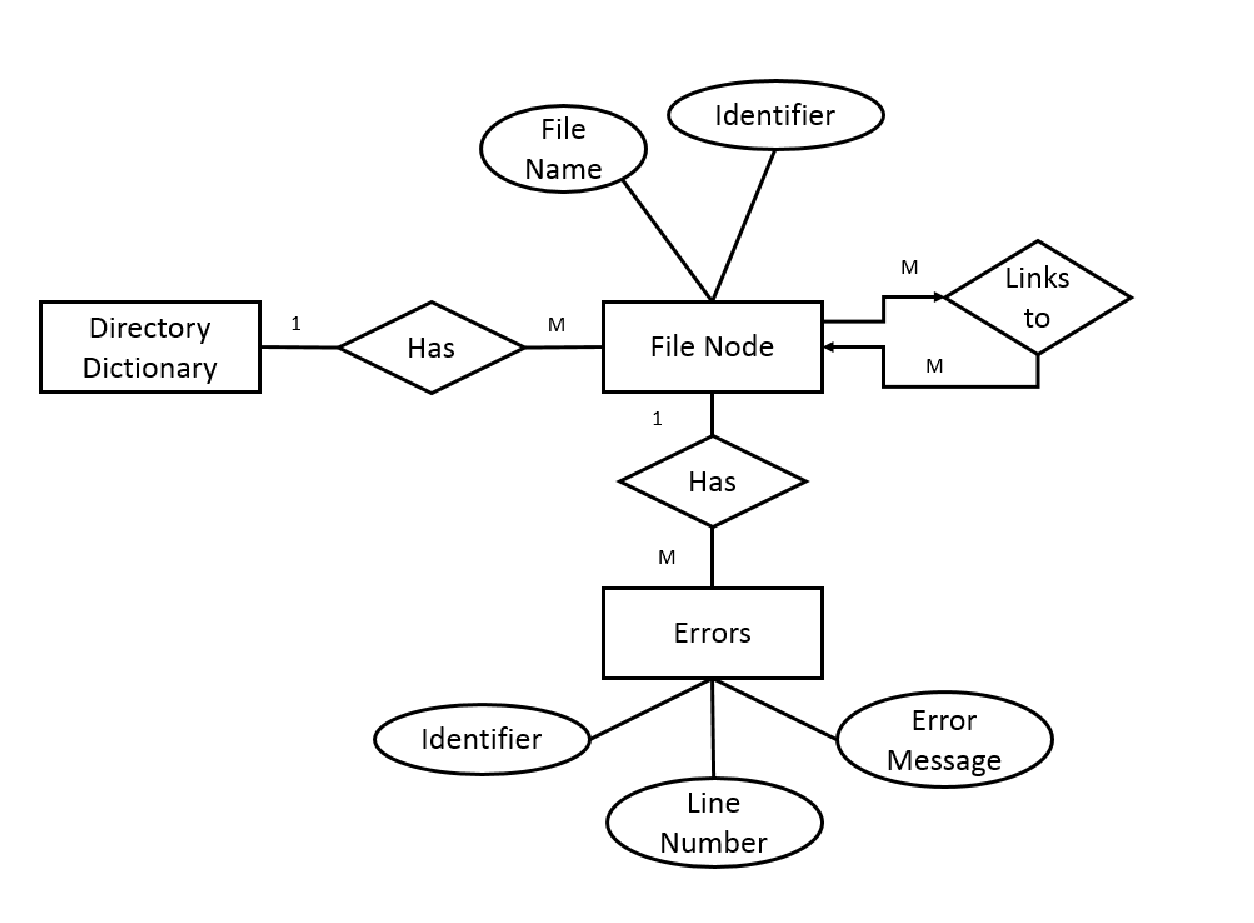
\includegraphics[width=300px]{InformationERDEPS.eps}
        \caption{A visual representation of the Datastructure.}
    \end{figure}
		
		
		
\section{Interface Viewpoints}
The Interface viewpoint provides information designers, programmers, and testers the means to know how
to correctly use the services provided by a design subject. This description includes the details of external
and internal interfaces not provided in the SRS. This viewpoint consists of a set of interface specifications
for each entity. 
\subsection{Design Concerns}
Identifies the interfaces that the components of the framework expose or require to achieve their
functionality. 
\subsection{Design Elements}


	\subsection{IDE}
		\subsubsection{Exposes}
			Opening the GUI give the user an interface in which they can interact and see the information that they are looking for from the Postal extension.
			That information includes the file structure and how they relate to eachother, as well as the possible errors. 
			The parsing of the file is the process that populates the information that is displayed in the UI.
		\subsubsection{Requires}
			These actions taken by the IDE require the use of the parser, the custom UI, and the event listeners.
	
	Parsers
		Exposes
			Parse 
		Requires
			Save File (IDE)
			Get Data (data structure)
	
\subsection{Data Structure}
		\subsubsection{Exposes}
		\begin{itemize}
			\item Get Data
			\\
			The data structure has its dictionary of file nodes updated when the Parser reparses the loaded project. 
			The data structure gets its data from the parser when Get Data is called.
		\subsubsection{Requires}
			\item Load Data (Files)
			\\
			The data structure will compare its updated data with the data stored in the JSON file. 
			In order for this to occur, the data structure must make use of JSON.parse and the deep object compare as part of the Load Data function.
			\item Parse (Parsers)
			\\
			The data structure will only have its data updated when the Parse function is called.
\subsection{UI}
		\subsubsection{Exposes}
		\begin{itemize}
			\item Error Navigation 
			When the user clicks on an error item in the error list, The UI component will interface with the VS Code IDE API in order to navigate the user's screen to the file and line number of the error.
			\item User-FileMap Interaction
			The User has several options to interface with the FIle Map. 
			When the user scrolls a mouse wheel, the file map will zoom and expand the size of the file nodes.
			If the user clicks and drags on the white space in the background of the file map, the GUI view will pan and render/discard file nodes that are off screen.
			If the user clicks on a file node and drags, the UI will simulate two dimensional physics and will warp the file map in response to the users movements.
			The three above features can all be achieved through the use of the vis.js API.
		\end{itemize}
		\begin{figure}
                 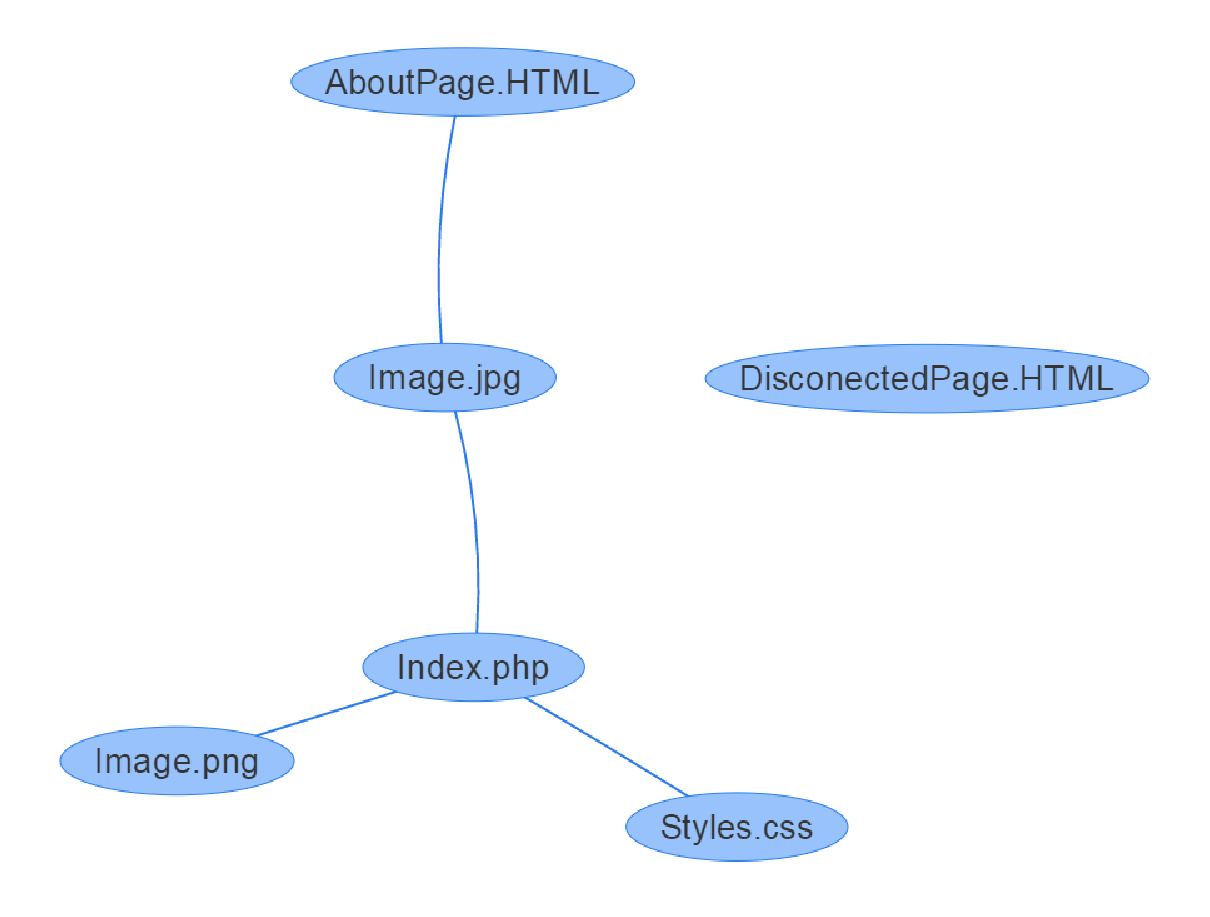
\includegraphics[width=300px]{UIMockupEPS.eps}
                 \caption{Mockup of the user interface}
                 \end{figure}
		\subsubsection{Requires}
		\begin{itemize}
			\item Get Data (data structure)
			\item Open GUI (IDE)
		\end{itemize}
		
	\subsection{Files}
		\subsubsection{Exposes}
		\begin{itemize}
			\item Load Data
			\\
			The JSON.parse function will be utilized to pull data from the JSON file.
			Once the information about the file nodes from the data structure are pulled from the JSON file, it will be compared to the current data structure values to identify which links or errors have changed.
			\item Save Data
			\\
			Once parsed data from the Parser is transfered to the data structure using the Get Data functionality, this data will be serialized into a JSON file with the JSON.stringify function built into JavaScript.
		\subsubsection{Requires}
		\begin{itemize}
			\item Get Data (data structure)
			\\
			It is necessary for the data structure to obtain data from the Parser each time it parses so that this data can, in turn, be saved to the JSON file.


% Annex A  Bibliography
% Annex B  Conforming design language description
% Annex C  Annex C Templates for an SDD

%\section{Conclusion}


\pagebreak
\bibliographystyle{IEEEtran}
\bibliography{design}

\end{document}
